% Ontologies for imaging data
% © 2026 Damien Goutte-Gattat
%
% This work is released under the Creative Commons
% Attribution-ShareAlike 4.0 International License. To view a copy of
% this license, visit https://creativecommons.org/licenses/by-sa/4.0/.
\usepackage{fontspec}
\usepackage{polyglossia}
\usepackage{tikz}
\usepackage{fancyvrb}

\setmainlanguage{english}
\usetheme{Boadilla}
\definecolor{gerbigreen}{RGB}{0,152,57}
\definecolor{gerbidarkgreen}{RGB}{0,146,55}
\definecolor{gerbilightgreen}{RGB}{212,235,220}
\usecolortheme[named=gerbidarkgreen]{structure}
\setbeamertemplate{navigation symbols}{}
\setbeamercovered{transparent}

\AtBeginSection{
  \begin{frame}{Outline}{}
    \tableofcontents[currentsection]
  \end{frame}
}
\graphicspath{{imgs/}{svgs/}}

% TikZ libraries and styles
\usetikzlibrary{positioning,shapes.geometric,graphs,graphdrawing,quotes,fit,overlay-beamer-styles}
\usegdlibrary{layered,trees}
\colorlet{GenericItem}{yellow!20!white}
\colorlet{GenericHighlight}{red!20!white}
\tikzset{Term/.style={draw,fill=yellow!20!white,font=\tiny\bfseries}}
\tikzset{RelationLabel/.style={shape=rectangle,fill=white,draw=black,thin,font=\tiny\bfseries,inner sep=1pt}}
\tikzset{File/.style={draw,fill=yellow!20!white,font=\tiny\ttfamily}}
\tikzset{Entity/.style={draw,fill=yellow!20!white,font=\scriptsize}}
\tikzset{Process/.style={draw,shape=ellipse,fill=blue!20!white,font=\scriptsize}}
\tikzset{IsARel/.style={draw=blue!80!white,very thick,arrows=->}}
\tikzset{PartOfRel/.style={draw=red!80!white,very thick,arrows=->}}
\tikzset{DevFromRel/.style={draw=green!80!white,very thick,arrows=->}}

\title{Ontologies for Imaging Data}
\author{Damien Goutte-Gattat}
\institute[German BioImaging e.V.]{
\includegraphics[width=4cm]{gerbi-logo}}
\date{Image Data Community Days 2026}

\hypersetup{pdfpagemode=UseNone,
  pdftitle={Ontologies for Imaging Data},
  pdfauthor={Damien Goutte-Gattat}}

\begin{document}

% Frontmatter

\mode<beamer>{
\begin{frame}
  \titlepage
\end{frame}
}


% Contents

\section{About ontologies}

\begin{frame}
  \frametitle{What is an ontology?}

  \begin{block}{}
    A knowledge classification of a domain, where the relationships
    between concepts are formally defined and logically related, which
    allows for computational reasoning.
  \end{block}

  \bigskip
  \begin{center}
    \begin{tikzpicture}[nodes={shape=rectangle,draw,fill=GenericItem}]
      \node (imaginaldisc) {imaginal disc};
      \node [right=of imaginaldisc] (multicellstr) {multi-cellular structure};
      \node [right=of multicellstr] (organismsdiv) {organism subdivision};
      \node [below=of imaginaldisc] (wingdisc)     {wing disc};
      \node [below=of multicellstr] (wing)         {wing};
      \node [below=of organismsdiv] (thorax)       {thorax};
      \node [below=of wingdisc]     (wingpouch)    {wing pouch};
      \node [below=of wing]         (wingblade)    {wing blade};
      \path [IsARel]     (imaginaldisc) -- (multicellstr) node[midway,RelationLabel] {is\_a};
      \path [IsARel]     (wingdisc) -- (imaginaldisc)     node[midway,RelationLabel] {is\_a};
      \path [IsARel]     (wing) -- (multicellstr)         node[midway,RelationLabel] {is\_a};
      \path [IsARel]     (thorax) -- (organismsdiv)       node[midway,RelationLabel] {is\_a};
      \path [PartOfRel]  (wing) -- (thorax)               node[midway,RelationLabel] {part\_of};
      \path [PartOfRel]  (wingblade) -- (wing)            node[midway,RelationLabel] {part\_of};
      \path [PartOfRel]  (wingpouch) -- (wingdisc)        node[midway,RelationLabel] {part\_of};
      \path [DevFromRel] (wing) -- (wingdisc)             node[midway,RelationLabel] {develops\_from};
      \path [DevFromRel] (wingblade) -- (wingpouch)       node[midway,RelationLabel] {develops\_from};
    \end{tikzpicture}
  \end{center}
\end{frame}

\begin{frame}[fragile]
  \frametitle{Controlled vocabularies, taxonomies, ontologies?}

  \begin{columns}[t]
    \begin{column}{.45\textwidth}
      \begin{block}{Controlled vocabulary}
        A flat list of terms, without any relationship between them.

\begin{Verbatim}
multicellular structure
organism subdivision
thorax
wing blade
wing disc
wing pouch
\end{Verbatim}
      \end{block}
    \end{column}
    \begin{column}{.45\textwidth}
      \begin{block}{Taxonomy}
        A controlled vocabulary where terms are connected through ``is
        a'' relationships.

\begin{Verbatim}
vertebrate
  mammal
    primate
      human
    rodent
      mouse
\end{Verbatim}
      \end{block}
    \end{column}
  \end{columns}
  
  \begin{block}{Ontology}
    A taxonomy where the relations between the terms are not limited
    to ``is a'', but are instead terms themselves.
  \end{block}

  \note{Dummy note for now.}
\end{frame}

\begin{frame}
  \frametitle{Biomedical ontologies}

  \begin{block}{Gene Ontology (1998)}
    Describes the functions, processes, and subcellular locations
    associated with genes and gene products.
  \end{block}

  \begin{block}{Open Bio-Ontologies (OBO) Foundry (2002)}
    A community of ontology developers agreeing on a shared set of
    principles.

    \bigskip
    From 60 bio-ontologies in 2007 to 245 in 2021.
    \begin{itemize}
      \item Gene Ontology (GO)
      \item Human Disease Ontology (DOID)
      \item \emph{Drosophila} Anatomy Ontology (FBbt)
      \item Zebrafish Phenotype Ontology (ZP)
      \item ...
      \item Biological Imaging Methods Ontology (FBbi)
    \end{itemize}
  \end{block}
\end{frame}


\section{About FBbi}

\begin{frame}
  \frametitle{A short history of FBbi}

  \begin{itemize}
    \item Initially created in the early 2000s at FlyBase to annotate
    the collection of fly images hosted at FlyBase
    \item Last release by FlyBase in 2005, when FlyBase stopped doing
    image curation
  \end{itemize}

  \bigskip
  \begin{itemize}
    \item Later successively maintained by
    \begin{itemize}
      \item Chris Woodcock for the Cell Image Library project;
      \item Willy Wong for the Center for Research in Biological Systems;
      \item David Osumi-Sutherland for the PhenoImageShare project.
    \end{itemize}
    \item All maintenance stopped at $\sim$2019.
  \end{itemize}

  \bigskip
  \begin{itemize}
    \item Maintenance resumed by German BioImaging for the FoundingGIDE
    project in early 2026.
  \end{itemize}
\end{frame}

\begin{frame}
  \frametitle{Overview of FBbi}

  \begin{columns}[t]
    \begin{column}{.45\textwidth}
      As of the January 2026 release:
      \begin{itemize}
        \item 649 classes
        \item 1 object property (``makes use of'')
      \end{itemize}
    \end{column}
    \begin{column}{.45\textwidth}
      Nine top-level terms:
      \begin{itemize}
        \item contrast-enhancing method
        \item detection method
        \item illumination method
        \item imaged parameter
        \item imaging method
        \item resolution-enhancing method
        \item sample preparation method
        \item source of contrast
        \item visualization method
      \end{itemize}
    \end{column}
  \end{columns}
\end{frame}


\section{Using FBbi}

\begin{frame}
  \frametitle{Browsing the ontology locally}

  Ontology editor of choice: Protégé (desktop application available for
  GNU/Linux, macOS, and Windows)
  \begin{itemize}
    \item Download it from \url{https://protege.stanford.edu}
    \item Then download FBbi itself from \url{http://purl.obolibrary.org/obo/fbbi.owl}
  \end{itemize}

  \begin{center}
    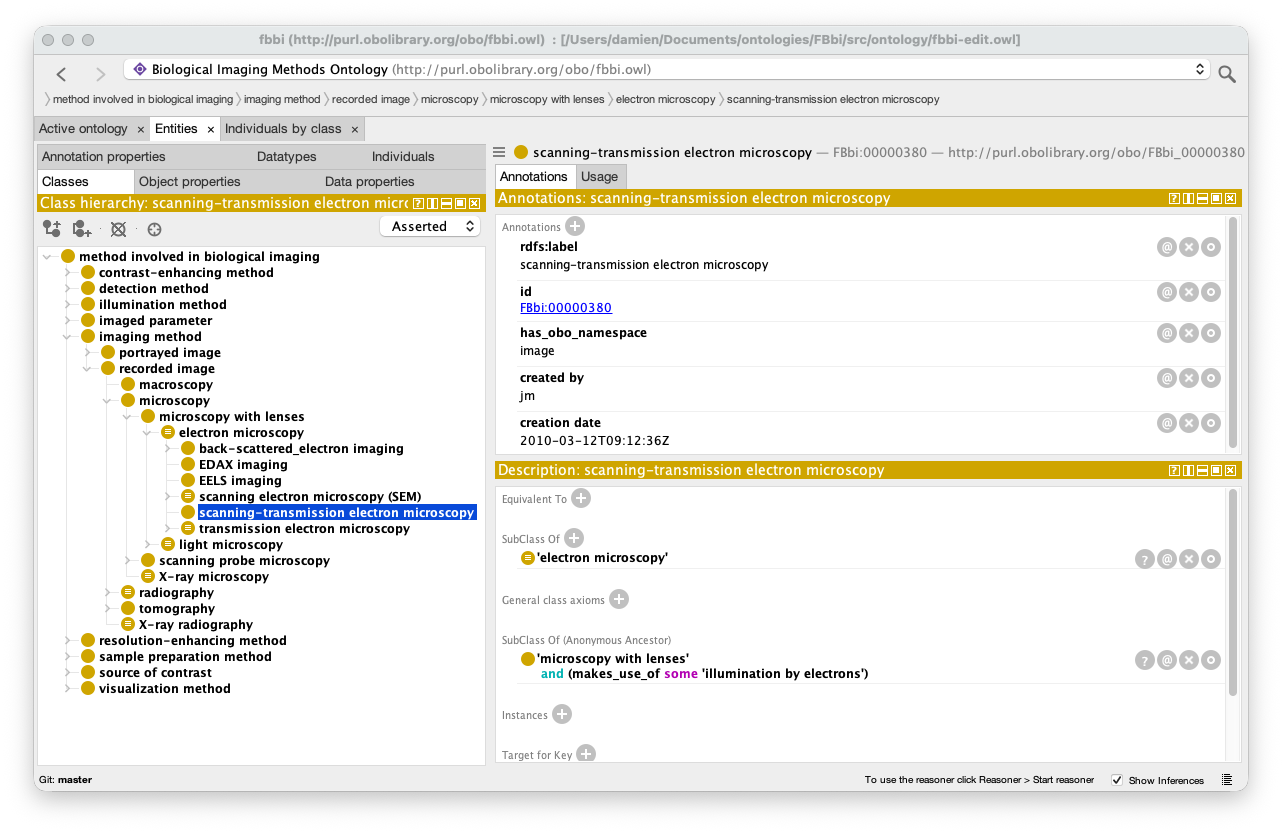
\includegraphics[scale=.16]{protege}
  \end{center}
\end{frame}

\begin{frame}
  \frametitle{Browsing the ontology online}

  Several ontology browsers are available online:
  \begin{itemize}
    \item Ontobee: \url{https://ontobee.org/ontology/FBbi}
    \item OLS: \url{https://www.ebi.ac.uk/ols4/ontologies/fbbi}
    \item AberOWL: \url{http://aber-owl.net/ontology/FBBI/\#/}
  \end{itemize}

  \begin{center}
    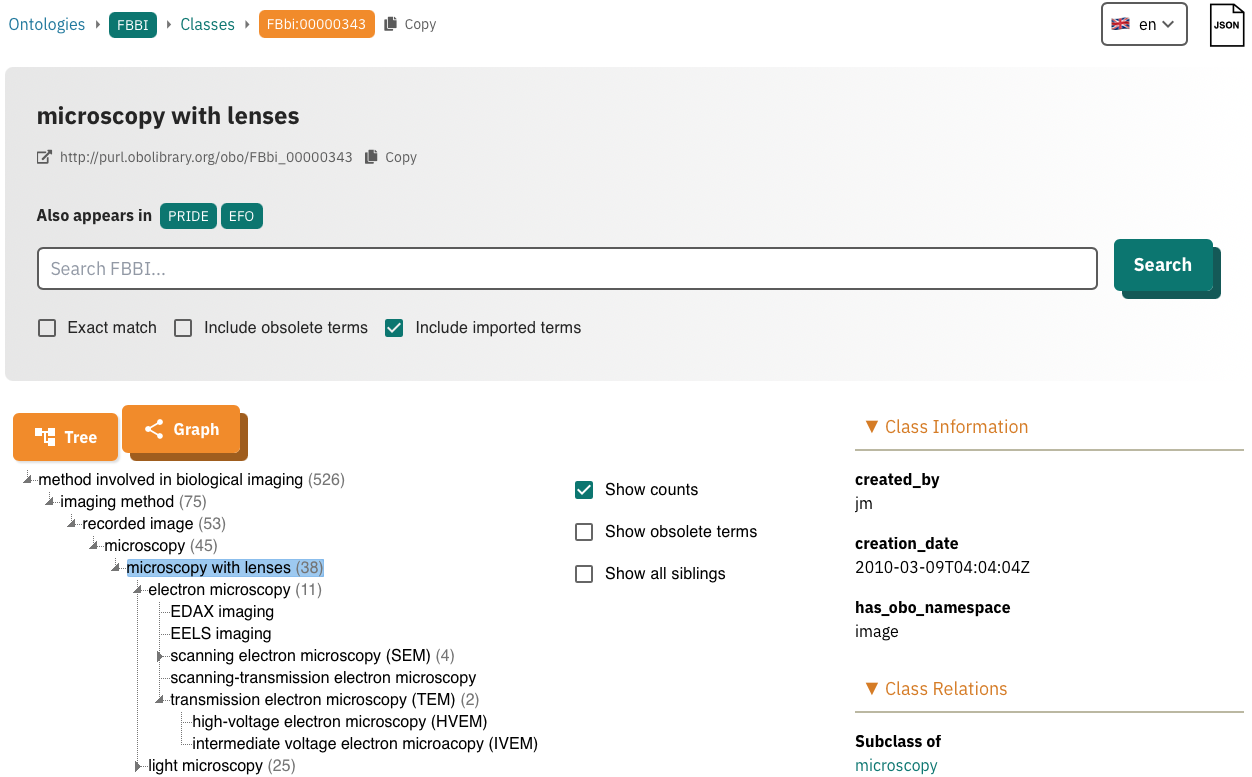
\includegraphics[scale=.14]{ols}
  \end{center}
\end{frame}


\section{Contributing to FBbi}

\begin{frame}
  \frametitle{You need something? Ask!}

  \begin{block}{}
    The easiest way for anyone to contribute to FBbi is to open a ticket
    on \url{https://github.com/foundingGIDE/fbbi/issues}.
  \end{block}

  \bigskip
  Whether you
  \begin{itemize}
    \item need of a term that is missing from the ontology,
    \item think that the definition of an existing term is perfectible
    \begin{itemize}
      \item (Definitions in an ontology are \emph{always} perfectible!),
    \end{itemize}
    \item think that a term is mis-classified,
    \item or have any other problem with the ontology as it currently
    is,
  \end{itemize}

  \bigskip
  Let us know about your problem so that we can fix it!

  \bigskip
  We are already aware of some problems but an ontology is always
  dependent on its users!
\end{frame}

\begin{frame}
  \frametitle{Want to contribute more directly?}

  What do you need to contribute?

  \begin{itemize}
    \item Software
    \begin{itemize}
      \item Protégé
      \item \href{https://github.com/INCATools/ontology-development-kit}{Ontology Development Kit}
    \end{itemize}
    \item Skills
    \begin{itemize}
      \item Familiarity with Git \& GitHub
      \item Familiarity with the command line
    \end{itemize}
    \item Documentation
    \begin{itemize}
      \item ``\href{https://oboacademy.github.io/obook/}{OBO Semantic Engineering Training}''
      \item Join the OBO community on Slack (\url{https://obo-communitygroup.slack.com})
    \end{itemize}
  \end{itemize}
\end{frame}


% Backmatter

\mode<beamer>{
\begin{frame}[noframenumbering]
  \frametitle{~}
\end{frame}

\begin{frame}[noframenumbering]
  \frametitle{About}

  \begin{block}{
\includegraphics[scale=.26]{ccbysa}\hspace{.2em}%
    2026 Damien Goutte-Gattat \texttt{<damien@gerbi-gmb.de>}}
    This presentation is released under the Creative Commons
    Attribution-ShareAlike 4.0 International License (CC BY-SA 4.0).
  \end{block}

  \begin{block}{Revision}\ttfamily\scriptsize
    \input{revision.tex}
  \end{block}
\end{frame}
}

\end{document}
